% Options for packages loaded elsewhere
\PassOptionsToPackage{unicode}{hyperref}
\PassOptionsToPackage{hyphens}{url}
\PassOptionsToPackage{dvipsnames,svgnames,x11names}{xcolor}
%
\documentclass[
  11pt,
]{krantz}
\usepackage{amsmath,amssymb}
\usepackage{lmodern}
\usepackage{iftex}
\ifPDFTeX
  \usepackage[T1]{fontenc}
  \usepackage[utf8]{inputenc}
  \usepackage{textcomp} % provide euro and other symbols
\else % if luatex or xetex
  \usepackage{unicode-math}
  \defaultfontfeatures{Scale=MatchLowercase}
  \defaultfontfeatures[\rmfamily]{Ligatures=TeX,Scale=1}
  \setmonofont[Scale=0.775]{MesloLGS NF}
\fi
% Use upquote if available, for straight quotes in verbatim environments
\IfFileExists{upquote.sty}{\usepackage{upquote}}{}
\IfFileExists{microtype.sty}{% use microtype if available
  \usepackage[]{microtype}
  \UseMicrotypeSet[protrusion]{basicmath} % disable protrusion for tt fonts
}{}
\makeatletter
\@ifundefined{KOMAClassName}{% if non-KOMA class
  \IfFileExists{parskip.sty}{%
    \usepackage{parskip}
  }{% else
    \setlength{\parindent}{0pt}
    \setlength{\parskip}{6pt plus 2pt minus 1pt}}
}{% if KOMA class
  \KOMAoptions{parskip=half}}
\makeatother
\usepackage{xcolor}
\IfFileExists{xurl.sty}{\usepackage{xurl}}{} % add URL line breaks if available
\IfFileExists{bookmark.sty}{\usepackage{bookmark}}{\usepackage{hyperref}}
\hypersetup{
  pdftitle={Data Science per psicologi},
  pdfauthor={Corrado Caudek},
  colorlinks=true,
  linkcolor={Maroon},
  filecolor={Maroon},
  citecolor={Blue},
  urlcolor={Blue},
  pdfcreator={LaTeX via pandoc}}
\urlstyle{same} % disable monospaced font for URLs
\usepackage{color}
\usepackage{fancyvrb}
\newcommand{\VerbBar}{|}
\newcommand{\VERB}{\Verb[commandchars=\\\{\}]}
\DefineVerbatimEnvironment{Highlighting}{Verbatim}{commandchars=\\\{\}}
% Add ',fontsize=\small' for more characters per line
\usepackage{framed}
\definecolor{shadecolor}{RGB}{248,248,248}
\newenvironment{Shaded}{\begin{snugshade}}{\end{snugshade}}
\newcommand{\AlertTok}[1]{\textcolor[rgb]{0.33,0.33,0.33}{#1}}
\newcommand{\AnnotationTok}[1]{\textcolor[rgb]{0.37,0.37,0.37}{\textbf{\textit{#1}}}}
\newcommand{\AttributeTok}[1]{\textcolor[rgb]{0.61,0.61,0.61}{#1}}
\newcommand{\BaseNTok}[1]{\textcolor[rgb]{0.06,0.06,0.06}{#1}}
\newcommand{\BuiltInTok}[1]{#1}
\newcommand{\CharTok}[1]{\textcolor[rgb]{0.5,0.5,0.5}{#1}}
\newcommand{\CommentTok}[1]{\textcolor[rgb]{0.37,0.37,0.37}{\textit{#1}}}
\newcommand{\CommentVarTok}[1]{\textcolor[rgb]{0.37,0.37,0.37}{\textbf{\textit{#1}}}}
\newcommand{\ConstantTok}[1]{\textcolor[rgb]{0,0,0}{#1}}
\newcommand{\ControlFlowTok}[1]{\textcolor[rgb]{0.27,0.27,0.27}{\textbf{#1}}}
\newcommand{\DataTypeTok}[1]{\textcolor[rgb]{0.27,0.27,0.27}{#1}}
\newcommand{\DecValTok}[1]{\textcolor[rgb]{0.06,0.06,0.06}{#1}}
\newcommand{\DocumentationTok}[1]{\textcolor[rgb]{0.37,0.37,0.37}{\textbf{\textit{#1}}}}
\newcommand{\ErrorTok}[1]{\textcolor[rgb]{0.14,0.14,0.14}{\textbf{#1}}}
\newcommand{\ExtensionTok}[1]{#1}
\newcommand{\FloatTok}[1]{\textcolor[rgb]{0.06,0.06,0.06}{#1}}
\newcommand{\FunctionTok}[1]{\textcolor[rgb]{0,0,0}{#1}}
\newcommand{\ImportTok}[1]{#1}
\newcommand{\InformationTok}[1]{\textcolor[rgb]{0.37,0.37,0.37}{\textbf{\textit{#1}}}}
\newcommand{\KeywordTok}[1]{\textcolor[rgb]{0.27,0.27,0.27}{\textbf{#1}}}
\newcommand{\NormalTok}[1]{#1}
\newcommand{\OperatorTok}[1]{\textcolor[rgb]{0.43,0.43,0.43}{\textbf{#1}}}
\newcommand{\OtherTok}[1]{\textcolor[rgb]{0.37,0.37,0.37}{#1}}
\newcommand{\PreprocessorTok}[1]{\textcolor[rgb]{0.37,0.37,0.37}{\textit{#1}}}
\newcommand{\RegionMarkerTok}[1]{#1}
\newcommand{\SpecialCharTok}[1]{\textcolor[rgb]{0,0,0}{#1}}
\newcommand{\SpecialStringTok}[1]{\textcolor[rgb]{0.5,0.5,0.5}{#1}}
\newcommand{\StringTok}[1]{\textcolor[rgb]{0.5,0.5,0.5}{#1}}
\newcommand{\VariableTok}[1]{\textcolor[rgb]{0,0,0}{#1}}
\newcommand{\VerbatimStringTok}[1]{\textcolor[rgb]{0.5,0.5,0.5}{#1}}
\newcommand{\WarningTok}[1]{\textcolor[rgb]{0.37,0.37,0.37}{\textbf{\textit{#1}}}}
\usepackage{longtable,booktabs,array}
\usepackage{calc} % for calculating minipage widths
% Correct order of tables after \paragraph or \subparagraph
\usepackage{etoolbox}
\makeatletter
\patchcmd\longtable{\par}{\if@noskipsec\mbox{}\fi\par}{}{}
\makeatother
% Allow footnotes in longtable head/foot
\IfFileExists{footnotehyper.sty}{\usepackage{footnotehyper}}{\usepackage{footnote}}
\makesavenoteenv{longtable}
\usepackage{graphicx}
\makeatletter
\def\maxwidth{\ifdim\Gin@nat@width>\linewidth\linewidth\else\Gin@nat@width\fi}
\def\maxheight{\ifdim\Gin@nat@height>\textheight\textheight\else\Gin@nat@height\fi}
\makeatother
% Scale images if necessary, so that they will not overflow the page
% margins by default, and it is still possible to overwrite the defaults
% using explicit options in \includegraphics[width, height, ...]{}
\setkeys{Gin}{width=\maxwidth,height=\maxheight,keepaspectratio}
% Set default figure placement to htbp
\makeatletter
\def\fps@figure{htbp}
\makeatother
\setlength{\emergencystretch}{3em} % prevent overfull lines
\providecommand{\tightlist}{%
  \setlength{\itemsep}{0pt}\setlength{\parskip}{0pt}}
\setcounter{secnumdepth}{5}
\usepackage{amsmath}
\usepackage{amssymb}
\usepackage{amsfonts}

\defaultfontfeatures{Scale=MatchLowercase}

\usepackage{booktabs}
\usepackage{longtable}
\usepackage[bf,singlelinecheck=off]{caption}

\usepackage{framed,color}
\definecolor{shadecolor}{RGB}{248,248,248}

\renewcommand{\textfraction}{0.05}
\renewcommand{\topfraction}{0.8}
\renewcommand{\bottomfraction}{0.8}
\renewcommand{\floatpagefraction}{0.75}

\renewenvironment{quote}{\begin{VF}}{\end{VF}}
\let\oldhref\href
\renewcommand{\href}[2]{#2\footnote{\url{#1}}}

\ifxetex
  \usepackage{letltxmacro}
  \setlength{\XeTeXLinkMargin}{1pt}
  \LetLtxMacro\SavedIncludeGraphics\includegraphics
  \def\includegraphics#1#{% #1 catches optional stuff (star/opt. arg.)
    \IncludeGraphicsAux{#1}%
  }%
  \newcommand*{\IncludeGraphicsAux}[2]{%
    \XeTeXLinkBox{%
      \SavedIncludeGraphics#1{#2}%
    }%
  }%
\fi

\makeatletter
\newenvironment{kframe}{%
\medskip{}
\setlength{\fboxsep}{.8em}
 \def\at@end@of@kframe{}%
 \ifinner\ifhmode%
  \def\at@end@of@kframe{\end{minipage}}%
  \begin{minipage}{\columnwidth}%
 \fi\fi%
 \def\FrameCommand##1{\hskip\@totalleftmargin \hskip-\fboxsep
 \colorbox{shadecolor}{##1}\hskip-\fboxsep
     % There is no \\@totalrightmargin, so:
     \hskip-\linewidth \hskip-\@totalleftmargin \hskip\columnwidth}%
 \MakeFramed {\advance\hsize-\width
   \@totalleftmargin\z@ \linewidth\hsize
   \@setminipage}}%
 {\par\unskip\endMakeFramed%
 \at@end@of@kframe}
\makeatother

\renewenvironment{Shaded}{\begin{kframe}}{\end{kframe}}

\usepackage{makeidx}
\makeindex

\urlstyle{tt}

\usepackage{amsthm}
\makeatletter
\def\thm@space@setup{%
  \thm@preskip=8pt plus 2pt minus 4pt
  \thm@postskip=\thm@preskip
}
\makeatother

\DeclareMathOperator{\V}{\mathbb{V}} % Define variance operator
\DeclareMathOperator{\Var}{\mathbb{V}} % Define variance operator
\DeclareMathOperator{\SD}{SD} % Define sd operator
\DeclareMathOperator{\Cov}{Cov} % Define covariance operator
\DeclareMathOperator{\Corr}{Corr} % Define correlation operator
\DeclareMathOperator{\Me}{Me} % Define mediane operator
\DeclareMathOperator{\Mo}{Mo} % Define mode operator

\DeclareMathOperator{\Bin}{Binomial} % Define binomial operator
\DeclareMathOperator{\Bernoulli}{Bernoulli} % Define Bernoulli operator
\DeclareMathOperator{\Ber}{\mathscr{B}} % Define Bernoulli operator
\DeclareMathOperator{\Poi}{Poisson} % Define Poisson operator
\DeclareMathOperator{\Uniform}{Uniform} % Define Uniform operator
\DeclareMathOperator{\Cauchy}{Cauchy} % Define Cauchy operator
\DeclareMathOperator{\B}{B} % beta function
% \mbox{B}(a, b) % beta function
% \mbox{Beta}(a, b) % beta distribution

\DeclareMathOperator{\elpd}{elpd} % Define elpd operator
\DeclareMathOperator{\lppd}{lppd} % Define lppd operator
\DeclareMathOperator{\LOO}{LOO} % Define LOO operator
\DeclareMathOperator{\argmin}{arg\,min} 
\DeclareMathOperator{\argmax}{arg\,max} 

\newcommand{\E}{\mathbb{E}} % Define expected value operator
\newcommand{\R}{\textsf{R}} % Define R programming language symbol
\newcommand{\Real}{\mathbb{R}} % Define real number operator
\newcommand{\Prob}{\mathscr{P}}
\newcommand{\indep}{\perp \!\!\! \perp}

\usepackage[
 labelfont=bf,
 font={small, it}
]{caption}
\usepackage{upquote} % print correct quotes in verbatim-environments
\usepackage{empheq}
\usepackage{xfrac}

\usepackage{polyglossia}
\setmainlanguage{italian}

\frontmatter
\ifLuaTeX
  \usepackage{selnolig}  % disable illegal ligatures
\fi
\usepackage[]{natbib}
\bibliographystyle{apalike}

\title{Data Science per psicologi}
\author{Corrado Caudek}
\date{2022-02-17}

\begin{document}
\maketitle

\cleardoublepage\newpage\thispagestyle{empty}\null
% \cleardoublepage\newpage\thispagestyle{empty}\null
%\cleardoublepage\newpage
\thispagestyle{empty}
\begin{center}
\Large{Psicometria -- AA 2021/2022}

\vskip20pt

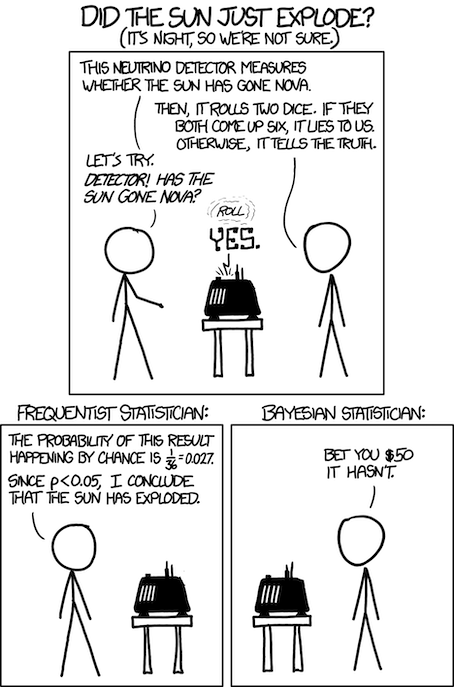
\includegraphics{images/frequentists_vs_bayesians.png}
\end{center}

\setlength{\abovedisplayskip}{-5pt}
\setlength{\abovedisplayshortskip}{-5pt}

{
\hypersetup{linkcolor=}
\setcounter{tocdepth}{2}
\tableofcontents
}
\listoffigures
\listoftables
\hypertarget{prefazione}{%
\chapter*{Prefazione}\label{prefazione}}


\emph{Data Science per psicologi} contiene il materiale delle lezioni dell'insegnamento di \emph{Psicometria B000286} (A.A. 2021/2022) rivolto agli studenti del primo anno del Corso di Laurea in Scienze e Tecniche Psicologiche dell'Università degli Studi di Firenze. \emph{Psicometria} si propone di fornire agli studenti un'introduzione all'analisi dei dati in psicologia. Le conoscenze/competenze che verranno sviluppate in questo insegnamento sono quelle della Data science, ovvero un insieme di conoscenze/competenze che si pongono all'intersezione tra statistica (ovvero, richiedono la capacità di comprendere teoremi statistici) e informatica (ovvero, richiedono la capacità di sapere utilizzare un software).

\hypertarget{la-psicologia-e-la-data-science}{%
\section*{La psicologia e la Data science}\label{la-psicologia-e-la-data-science}}


Sembra sensato spendere due parole su un tema che è importante per gli studenti: quello indicato dal titolo di questo Capitolo. È ovvio che agli studenti di psicologia la statistica non piace. Se piacesse, forse studierebbero Data science e non psicologia; ma non lo fanno. Di conseguenza, gli studenti di psicologia si chiedono: ``perché dobbiamo perdere tanto tempo a studiare queste cose quando in realtà quello che ci interessa è tutt'altro?'' Questa è una bella domanda.

C'è una ragione molto semplice che dovrebbe farci capire perché la Data science è così importante per la psicologia. Infatti, a ben pensarci, la psicologia è una disciplina intrinsecamente statistica, se per statistica intendiamo quella disciplina che studia la variazione delle caratteristiche degli individui nella popolazione. La psicologia studia \emph{gli individui} ed è proprio la variabilità inter- e intra-individuale ciò che vogliamo descrivere e, in certi casi, predire. In questo senso, la psicologia è molto diversa dall'ingegneria, per esempio. Le proprietà di un determinato ponte sotto certe condizioni, ad esempio, sono molto simili a quelle di un altro ponte, sotto le medesime condizioni. Quindi, per un ingegnere la statistica è poco importante: le proprietà dei materiali sono unicamente dipendenti dalla loro composizione e restano costanti. Ma lo stesso non può dirsi degli individui: ogni individuo è unico e cambia nel tempo. E le variazioni tra gli individui, e di un individuo nel tempo, sono l'oggetto di studio proprio della psicologia: è dunque chiaro che i problemi che la psicologia si pone sono molto diversi da quelli affrontati, per esempio, dagli ingegneri. Questa è la ragione per cui abbiamo tanto bisogno della Data science in psicologia: perché la Data science ci consente di descrivere la variazione e il cambiamento. E queste sono appunto le caratteristiche di base dei fenomeni psicologici.

Sono sicuro che, leggendo queste righe, a molti studenti sarà venuta in mente la seguente domanda: perché non chiediamo a qualche esperto di fare il ``lavoro sporco'' (ovvero le analisi statistiche) per noi, mentre noi (gli psicologi) ci occupiamo solo di ciò che ci interessa, ovvero dei problemi psicologici slegati dai dettagli ``tecnici'' della Data science? La risposta a questa domanda è che non è possibile progettare uno studio psicologico sensato senza avere almeno una comprensione rudimentale della Data science. Le tematiche della Data science non possono essere ignorate né dai ricercatori in psicologia né da coloro che svolgono la professione di psicologo al di fuori dell'Università. Infatti, anche i professionisti al di fuori dall'università non possono fare a meno di leggere la letteratura psicologica più recente: il continuo aggiornamento delle conoscenze è infatti richiesto dalla deontologia della professione. Ma per potere fare questo è necessario conoscere un bel po' di Data science! Basta aprire a caso una rivista specialistica di psicologia per rendersi conto di quanto ciò sia vero: gli articoli che riportano i risultati delle ricerche psicologiche sono zeppi di analisi statistiche e di modelli formali. E la comprensione della letteratura psicologica rappresenta un requisito minimo nel bagaglio professionale dello psicologo.

Le considerazioni precedenti cercano di chiarire il seguente punto: la Data science non è qualcosa da studiare a malincuore, in un singolo insegnamento universitario, per poi poterla tranquillamente dimenticare. Nel bene e nel male, gli psicologi usano gli strumenti della Data science in tantissimi ambiti della loro attività professionale: in particolare quando costruiscono, somministrano e interpretano i test psicometrici. È dunque chiaro che possedere delle solide basi di Data science è un tassello imprescindibile del bagaglio professionale dello psicologo. In questo insegnamento verrano trattati i temi base della Data science e verrà adottato un punto di vista bayesiano, che corrisponde all'approccio più recente e sempre più diffuso in psicologia.

\hypertarget{come-studiare}{%
\section*{Come studiare}\label{come-studiare}}


Il giusto metodo di studio per prepararsi all'esame di Psicometria è quello di seguire attivamente le lezioni, assimilare i concetti via via che essi vengono presentati e verificare in autonomia le procedure presentate a lezione. Incoraggio gli studenti a farmi domande per chiarire ciò che non è stato capito appieno. Incoraggio gli studenti a utilizzare i forum attivi su Moodle e, soprattutto, a svolgere gli esercizi proposti su Moodle. I problemi forniti su Moodle rappresentano il livello di difficoltà richiesto per superare l'esame e consentono allo studente di comprendere se le competenze sviluppate fino a quel punto sono sufficienti rispetto alle richieste dell'esame.

La prima fase dello studio, che è sicuramente individuale, è quella in cui è necessario acquisire le conoscenze teoriche relative ai problemi che saranno presentati all'esame. La seconda fase di studio, che può essere facilitata da scambi con altri e da incontri di gruppo, porta ad acquisire la capacità di applicare le conoscenze: è necessario capire come usare un software (\(\textsf{R}\)) per applicare i concetti statistici alla specifica situazione del problema che si vuole risolvere. Le due fasi non sono però separate: il saper fare molto spesso ci aiuta a capire meglio.

\hypertarget{sviluppare-un-metodo-di-studio-efficace}{%
\section*{Sviluppare un metodo di studio efficace}\label{sviluppare-un-metodo-di-studio-efficace}}


Avendo insegnato molte volte in passato un corso introduttivo di analisi dei dati ho notato nel corso degli anni che gli studenti con l'atteggiamento mentale che descriverò qui sotto generalmente ottengono ottimi risultati. Alcuni studenti sviluppano naturalmente questo approccio allo studio, ma altri hanno bisogno di fare uno sforzo per maturarlo. Fornisco qui sotto una breve descrizione del ``metodo di studio'' che, nella mia esperienza, è il più efficace per affrontare le richieste di questo insegnamento.

\begin{itemize}
\tightlist
\item
  Dedicate un tempo sufficiente al materiale di base, apparentemente facile; assicuratevi di averlo capito bene. Cercate le lacune nella vostra comprensione. Leggere presentazioni diverse dello stesso materiale (in libri o articoli diversi) può fornire nuove intuizioni.
\item
  Gli errori che facciamo sono i nostri migliori maestri. Istintivamente cerchiamo di dimenticare subito i nostri errori. Ma il miglior modo di imparare è apprendere dagli errori che commettiamo. In questo senso, una soluzione corretta è meno utile di una soluzione sbagliata. Quando commettiamo un errore questo ci fornisce un'informazione importante: ci fa capire qual è il materiale di studio sul quale dobbiamo ritornare e che dobbiamo capire meglio.
\item
  C'è ovviamente un aspetto ``psicologico'' nello studio. Quando un esercizio o problema ci sembra incomprensibile, la cosa migliore da fare è dire: ``mi arrendo'', ``non ho idea di cosa fare!''. Questo ci rilassa: ci siamo già arresi, quindi non abbiamo niente da perdere, non dobbiamo più preoccuparci. Ma non dobbiamo fermarci qui. Le cose ``migliori'' che faccio (se ci sono) le faccio quando non ho voglia di lavorare. Alle volte, quando c'è qualcosa che non so fare e non ho idea di come affontare, mi dico: ``oggi non ho proprio voglia di fare fatica'', non ho voglia di mettermi nello stato mentale per cui ``in 10 minuti devo risolvere il problema perché dopo devo fare altre cose''. Però ho voglia di \emph{divertirmi} con quel problema e allora mi dedico a qualche aspetto ``marginale'' del problema, che so come affrontare, oppure considero l'aspetto più difficile del problema, quello che non so come risolvere, ma invece di cercare di risolverlo, guardo come altre persone hanno affrontato problemi simili, opppure lo stesso problema in un altro contesto. Non mi pongo l'obiettivo ``risolvi il problema in 10 minuti'', ma invece quello di farmi un'idea ``generale'' del problema, o quello di capire un caso più specifico e più semplice del problema. Senza nessuna pressione. Infatti, in quel momento ho deciso di non lavorare (ovvero, di non fare fatica). Va benissimo se ``parto per la tangente'', ovvero se mi metto a leggere del materiale che sembra avere poco a che fare con il problema centrale (le nostre intuizioni e la nostra curiosità solitamente ci indirizzano sulla strada giusta). Quando faccio così, molto spesso trovo la soluzione del problema che mi ero posto e, paradossalmente, la trovo in un tempo minore di quello che, in precedenza, avevo dedicato a ``lavorare'' al problema. Allora perché non faccio sempre così? C'è ovviamente l'aspetto dei ``10 minuti'' che non è sempre facile da dimenticare. Sotto pressione, possiamo solo agire in maniera automatica, ovvero possiamo solo applicare qualcosa che già sappiamo fare. Ma se dobbiamo imparare qualcosa di nuovo, la pressione è un impedimento.
\item
  È utile farsi da soli delle domande sugli argomenti trattati, senza limitarsi a cercare di risolvere gli esercizi che vengono assegnati. Quando studio qualcosa mi viene in mente: ``se questo è vero, allora deve succedere quest'altra cosa''. Allora verifico se questo è vero, di solito con una simulazione. Se i risultati della simulazione sono quelli che mi aspetto, allora vuol dire che ho capito. Se i risultati sono diversi da quelli che mi aspettavo, allora mi rendo conto di non avere capito e ritorno indietro a studiare con più attenzione la teoria che pensavo di avere capito -- e ovviamente mi rendo conto che c'era un aspetto che avevo frainteso. Questo tipo di verifica è qualcosa che dobbiamo fare da soli, in prima persona: nessun altro può fare questo al posto nostro.
\item
  Non aspettatevi di capire tutto la prima volta che incontrate un argomento nuovo.\footnote{Ricordatevi inoltre che gli individui tendono a sottostimare la propria capacità di apprendere \citep{horn2021underestimating}.} È utile farsi una nota mentalmente delle lacune nella vostra comprensione e tornare su di esse in seguito per carcare di colmarle. L'atteggiamento naturale, quando non capiamo i dettagli di qualcosa, è quello di pensare: ``non importa, ho capito in maniera approssimativa questo punto, non devo preoccuparmi del resto''. Ma in realtà non è vero: se la nostra comprensione è superficiale, quando il problema verrà presentato in una nuova forma, non riusciremo a risolverlo. Per cui i dubbi che ci vengono quando studiamo qualcosa sono il nostro alleato più prezioso: ci dicono esattamente quali sono gli aspetti che dobbiamo approfondire per potere migliorare la nostra preparazione.
\item
  È utile sviluppare una visione d'insieme degli argomenti trattati, capire l'obiettivo generale che si vuole raggiungere e avere chiaro il contributo che i vari pezzi di informazione forniscono al raggiungimento di tale obiettivo. Questa organizzazione mentale del materiale di studio facilita la comprensione. È estremamente utile creare degli schemi di ciò che si sta studiando. Non aspettate che sia io a fornirvi un riepilogo di ciò che dovete imparare: sviluppate da soli tali schemi e tali riassunti.
\item
  Tutti noi dobbiamo imparare l'arte di trovare le informazioni, non solo nel caso di questo insegnamento. Quando vi trovate di fronte a qualcosa che non capite, o ottenete un oscuro messaggio di errore da un software, ricordatevi: ``Google is your friend''!
\end{itemize}

\begin{flushright}
Corrado Caudek\\
Marzo 2022 \end{flushright}

\mainmatter

\hypertarget{part-il-modello-lineare}{%
\part{Il modello lineare}\label{part-il-modello-lineare}}

\hypertarget{regr-models-intro}{%
\chapter{Introduzione}\label{regr-models-intro}}

Lo scopo della ricerca è trovare le associazioni tra le variabili e fare confronti fra le condizioni sperimentali. Nel caso della psicologia, il ricercatore vuole scoprire le leggi generali che descrivono le relazioni tra i costrutti psicologici e le relazioni che intercorrono tra i fenomeni psicologici e quelli non psicologici (sociali, economici, storici, \ldots). Abbiamo già visto come la correlazione di Pearson sia uno strumento adatto a questo scopo. Infatti, essa ci informa sulla direzione e sull'intensità della relazione lineare tra due variabili. Tuttavia, la correlazione non è sufficiente, in quanto il ricercatore ha a disposizione solo i dati di un campione, mentre vorrebbe descrivere la relazione tra le variabili nella popolazione. A causa della variabilità campionaria, le proprietà dei campioni sono necessariamente diverse da quelle della popolazione: ciò che si può osservare nella popolazione potrebbe non emergere nel campione e, al contrario, il campione manifesta caratteristiche che non sono necessariamente presenti nella popolazione. È dunque necessario chiarire, dal punto di vista statistico, il legame che intercorre tra le proprietà del campione e le proprietà della popolazione da cui esso è stato estratto. Il modello lineare utilizza la funzione matematica più semplice per descrivere la relazione fra due variabili, ovvero la funzione lineare. In questo Capitolo vedremo come si possa fare inferenza sulla relazione tra due variabili mediante il modello lineare bayesiano. Inizieremo a descrivere le proprietà geometriche della funzione lineare per poi utilizzare questa semplice funzione per costruire un modello statistico secondo un approccio bayesiano.

\hypertarget{la-funzione-lineare}{%
\section{La funzione lineare}\label{la-funzione-lineare}}

Iniziamo con un ripasso sulla funzione di lineare. Si chiama \emph{funzione lineare} una funzione del tipo

\begin{equation}
f(x) = a + b x,
\end{equation}

dove \(a\) e \(b\) sono delle costanti. Il grafico di tale funzione è una retta di cui il parametro \(b\) è detto \emph{coefficiente angolare} e il parametro \(a\) è detto \emph{intercetta} con l'asse delle \(y\) {[}infatti, la retta interseca l'asse \(y\) nel punto \((0,a)\), se \(b \neq 0\){]}.

Per assegnare un'interpretazione geometrica alle costanti \(a\) e \(b\) si consideri la funzione

\begin{equation}
y = b x.
\end{equation}

Tale funzione rappresenta un caso particolare, ovvero quello della \emph{proporzionalità diretta} tra \(x\) e \(y\). Il caso generale della linearità

\begin{equation}
y = a + b x
\end{equation}

non fa altro che sommare una costante \(a\) a ciascuno dei valori \(y = b x\). Nella funzione lineare \(y = a + b x\), se \(b\) è positivo allora \(y\) aumenta al crescere di \(x\); se \(b\) è negativo allora \(y\) diminuisce al crescere di \(x\); se \(b=0\) la retta è orizzontale, ovvero \(y\) non muta al variare di \(x\).

Consideriamo ora il coefficiente \(b\). Si consideri un punto \(x_0\) e un incremento arbitrario \(\varepsilon\) come indicato nella figura \ref{fig:linearfunction}. Le differenze \(\Delta x = (x_0 + \varepsilon) - x_0\) e \(\Delta y = f(x_0 + \varepsilon) - f(x_0)\) sono detti \emph{incrementi} di \(x\) e \(y\). Il coefficiente angolare \(b\) è uguale al rapporto

\begin{equation}
    b = \frac{\Delta y}{\Delta x} = \frac{f(x_0 + \varepsilon) - f(x_0)}{(x_0 + \varepsilon) - x_0},
\end{equation}

indipendentemente dalla grandezza degli incrementi \(\Delta x\) e \(\Delta y\). Il modo più semplice per assegnare un'interpretazione geometrica al coefficiente angolare (o pendenza) della retta è dunque quello di porre \(\Delta x = 1\). In tali circostanze infatti \(b = \Delta y\).

\begin{figure}

{\centering 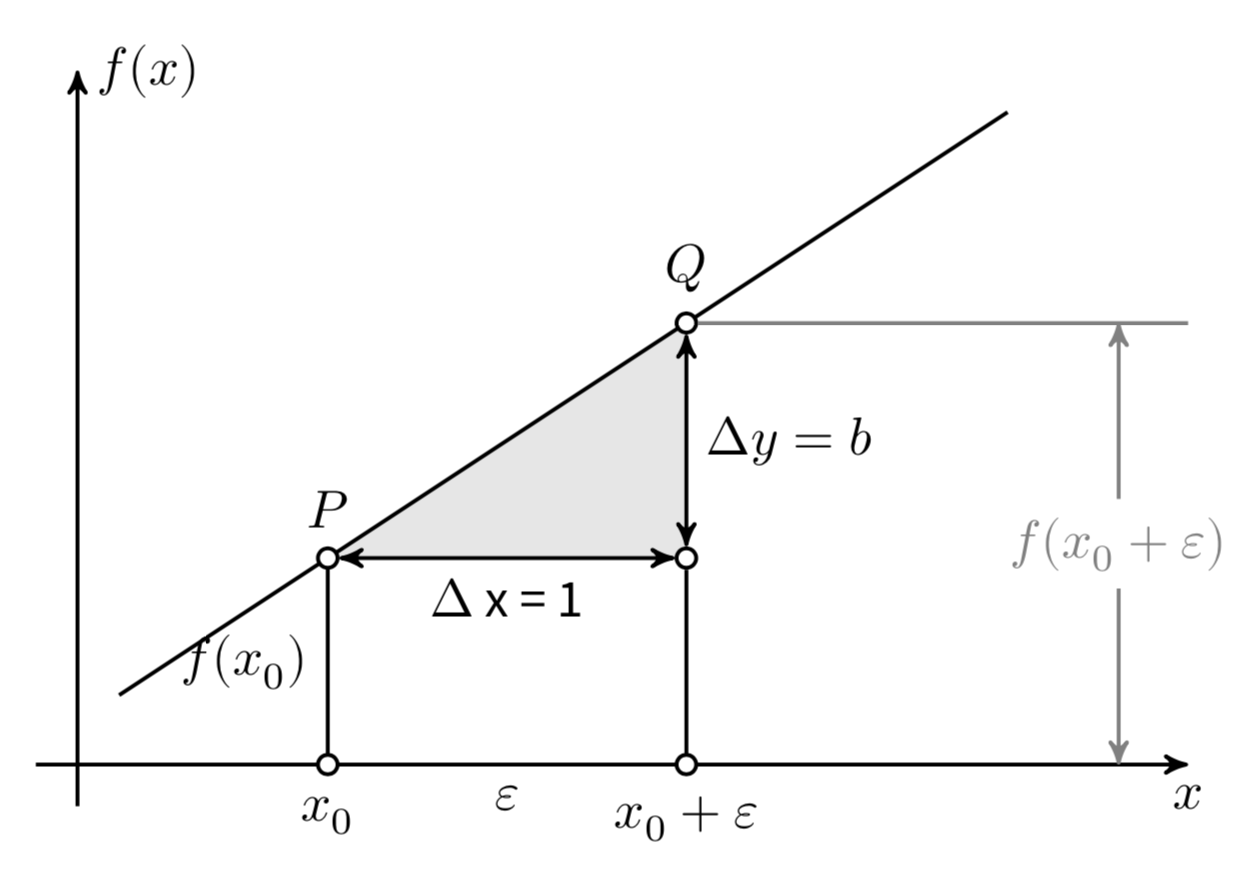
\includegraphics[width=0.75\linewidth]{images/linear_function} 

}

\caption{La funzione lineare $y = a + bx$.}\label{fig:linearfunction}
\end{figure}

\hypertarget{una-media-per-ciascuna-osservazione}{%
\section{Una media per ciascuna osservazione}\label{una-media-per-ciascuna-osservazione}}

In precedenza abbiamo visto come sia possibile stimare i parametri di un modello bayesiano nel quale le osservazioni sono indipendenti e identicamente distribuite secondo una densità gaussiana,

\begin{equation}
Y_i \stackrel{i.i.d.}{\sim} \mathcal{N}(\mu, \sigma), \quad i = 1, \dots, n.
\label{eq:normalsamplingmodel}
\end{equation}

Il modello \eqref{eq:normalsamplingmodel} assume che ogni \(Y_i\) sia la realizzazione di una v.c. descritta da una \(\mathcal{N}(\mu, \sigma^2)\). Da un punto di vista bayesiano, si assegnano distribuzioni a priori ai parametri \(\mu\) e \(\sigma\), si genera la verosimiglianza in base ai dati osservati e, con queste informazioni, si generano le distribuzione a posteriori dei parametri \citep{gelman2020regression}:

\begin{align}
Y_i \mid \mu, \sigma & \stackrel{iid}{\sim} \mathcal{N}(\mu, \sigma^2)\notag\\
\mu       & \sim \mathcal{N}(\mu_0, \tau^2) \notag\\
\sigma    & \sim \Cauchy(x_0, \gamma) \notag
\end{align}

È comune però che vengano registrate altre variabili \(x_i\) che possono essere associate alla risposta di interesse \(y_i\). La variabile \(x_i\) viene chiamata \emph{predittore} (o variabile indipendente) in quanto il ricercatore è tipicamente interessato a predire il valore \(y_i\) a partire da \(x_i\). Come si può estende il modello \eqref{eq:normalsamplingmodel} per lo studio della possibile relazione tra \(y_i\) e \(x_i\)?

Il modello \eqref{eq:normalsamplingmodel} assume una media \(\mu\) comune per ciascuna osservazione \(Y_i\). Dal momento che desideriamo introdurre una nuova variabile \(x_i\) che assume un diverso valore per ciascuna osservazione \(y_i\), il modello \eqref{eq:normalsamplingmodel} può essere modificato in modo che la media comune \(\mu\) venga sostituita da una media \(\mu_i\) specifica a ciascuna osservazione \(i\)-esima:

\begin{equation}
Y_i \mid \mu_i, \sigma \stackrel{ind}{\sim} \mathcal{N}(\mu_i, \sigma), \quad i = 1, \dots, n.
\label{eq:normalsamplinglinearmodel}
\end{equation}

Si noti che le osservazioni \(Y_1, \dots, Y_n\) non sono più identicamente distribuite poiché hanno medie diverse, ma sono ancora indipendenti come indicato dalla notazione \texttt{ind} posta sopra il simbolo \(\sim\) nella \eqref{eq:normalsamplinglinearmodel}.

\hypertarget{relazione-lineare-tra-la-media-y-mid-x-e-il-predittore}{%
\subsection{\texorpdfstring{Relazione lineare tra la media \(y \mid x\) e il predittore}{Relazione lineare tra la media y \textbackslash mid x e il predittore}}\label{relazione-lineare-tra-la-media-y-mid-x-e-il-predittore}}

L'approccio che consente di mettere in relazione un predittore \(x_i\) con la risposta \(Y_i\) è quello di assumere che la media di ciascuna \(Y_i\), ovvero \(\mu_i\), sia una funzione lineare del predittore \(x_i\). Una tale relazione lineare è scritta come

\begin{equation}
\mu_i = \beta_0 + \beta_ 1 x_i, \quad i = 1, \dots, n.
\label{eq:regmodel}
\end{equation}

Nella \eqref{eq:regmodel}, ciascuna \(x_i\) è una costante nota (ecco perché viene usata una lettera minuscola per la \(x\)) e \(\beta_0\) e \(\beta_ 1\) sono parametri incogniti. Questi parametri rappresentano l'intercetta e la pendenza della retta di regressione e sono delle variabili casuali.\footnote{Una notazione alternativa per tali parametri è \(\alpha\), \(\beta\), anziché \(\beta_0\), \(\beta_ 1\).} L'inferenza bayesiana procede assegnando una distribuzione a priori a \(\beta_0\) e a \(\beta_ 1\) e si esegue l'inferenza riassumendo la distribuzione a posteriori di questi parametri.

Nel modello \eqref{eq:regmodel}, la funzione lineare \(\beta_0 + \beta_ 1 x_i\) è interpretata come il valore atteso della \(Y_i\) per ciascun valore \(x_i\), mentre l'intercetta \(\beta_0\) rappresenta il valore atteso della \(Y_i\) quando \(x_i = 0\). Il parametro \(\beta_ 1\) (pendenza) rappresenta invece l'aumento medio della \(Y_i\) quando \(x_i\) aumenta di un'unità. È importante notare che la relazione lineare \eqref{eq:normalsamplinglinearmodel} di parametri \(\beta_0\) e \(\beta_ 1\) descrive l'associazione tra \emph{la media} \(\mu_i\) e il predittore \(x_i\). In altri termini, tale relazione lineare ci fornisce una predizione sul valore medio \(\mu_i\), non sul valore \emph{effettivo} \(Y_i\).

\hypertarget{il-modello-lineare}{%
\subsection{Il modello lineare}\label{il-modello-lineare}}

Sostituendo la \eqref{eq:regmodel} nella \eqref{eq:normalsamplinglinearmodel} otteniamo il modello lineare:

\begin{equation}
Y_i \mid \beta_0, \beta_ 1, \sigma \stackrel{ind}{\sim} \mathcal{N}(\beta_0 + \beta_ 1 x_i, \sigma), \quad i = 1, \dots, n.
\label{eq:samplinglinearmodel}
\end{equation}

Questo è un caso speciale del modello di campionamento Normale, dove le \(Y_i\) seguono indipendentemente una densità Normale con una media (\(\beta_0 + \beta_ 1 x_i\)) specifica per ciascuna osservazione e con una deviazione standard (\(\sigma\)) comune a tutte le osservazioni. Poiché include un solo predittore (\(x\)), questo modello è comunemente chiamato \emph{modello di regressione lineare semplice}.

\begin{center}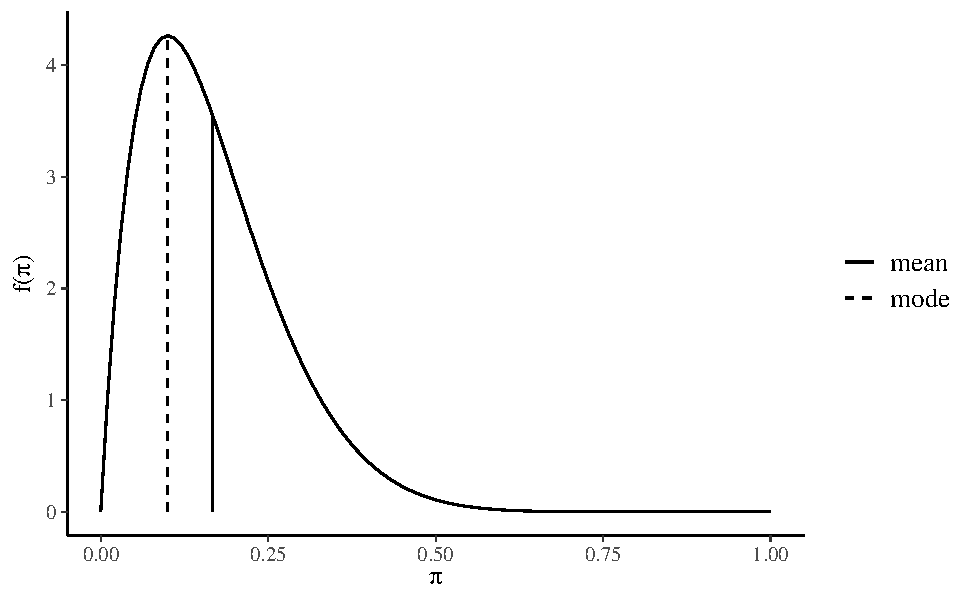
\includegraphics{ds4psy_files/figure-latex/unnamed-chunk-2-1} \end{center}

\hypertarget{commenti-e-considerazioni-finali}{%
\section*{Commenti e considerazioni finali}\label{commenti-e-considerazioni-finali}}


Il modello lineare semplice viene usato per descrivere la relazione tra due variabili e per determinare il segno e l'intensità di tale relazione. Inoltre, il modello lineare ci consente di prevedere il valore della variabile dipendente in base ai valori della variabile indipendente.

\hypertarget{reg-lin-stan}{%
\chapter{Modello lineare in Stan}\label{reg-lin-stan}}

Mostreremo qui come sia possibile usare il linguaggio probabilistico Stan per la stima dei parametri del modello di regressione. Vedremo anche come interpretare i risultati dell'analisi bayesiana (si vedano anche le Appendici \ref{regr-ml} e \ref{regr-lin-frequentista}).

\hypertarget{una-distribuzione-a-priori-debolmente-informativa}{%
\section{Una distribuzione a priori debolmente informativa}\label{una-distribuzione-a-priori-debolmente-informativa}}

Per implementare l'approccio bayesiano è necessario assegnare una distribuzione a priori ai parametri. Nel contesto del modello di regressione è desiderabile scegliere distribuzioni a priori che abbiano uno scarso impatto sulla distribuzione a posteriori.

Supponiamo che le nostre credenza a priori sui parametri del modello, \(\beta_0\), \(\beta_1\) e \(\sigma\) siano tra loro indipendenti. Allora possiamo scrivere la distribuzione congiunta dei parametri nel modo seguente:

\[
p(\beta_0, \beta_1, \sigma) = p(\beta_0)p(\beta_1)p(\sigma).
\]

Possiamo dunque assumere \(\beta_0 \sim \mathcal{N}(\mu_0, s_0)\) e \(\beta_1 \sim \mathcal{N}(\mu_1, s_1)\). Per \(\sigma\) possiamo assumere \(\sigma \sim \mbox{Cauchy}(a, b)\). Moltiplicando la verosimiglianza

\[
\prod_{i=1}^n p(y_i \mid x_i; \beta_0, \beta_1, \sigma^2) = \prod_{i=1}^n \frac{1}{\sqrt{2 \pi \sigma^2}}e^{-\frac{(y_i-(\beta_0+\beta_1 x_i))^2}{2\sigma^2}}
\]

per le distribuzioni a priori dei parametri, si ottiene la distribuzione a posteriori. Tuttavia, tale distribuzione non è risolvibile per via analitica. È dunque necessario utilizzare un algoritmo MCMC per ottenere una sequenza di campioni casuali dalla distribuzione a posteriori.

\hypertarget{linguaggio-stan}{%
\section{Linguaggio Stan}\label{linguaggio-stan}}

Leggiamo in \(\textsf{R}\) il dataset \texttt{kidiq}:

\begin{Shaded}
\begin{Highlighting}[]
\FunctionTok{library}\NormalTok{(}\StringTok{"rio"}\NormalTok{)}
\NormalTok{df }\OtherTok{\textless{}{-}}\NormalTok{ rio}\SpecialCharTok{::}\FunctionTok{import}\NormalTok{(here}\SpecialCharTok{::}\FunctionTok{here}\NormalTok{(}\StringTok{"data"}\NormalTok{, }\StringTok{"kidiq.dta"}\NormalTok{))}
\FunctionTok{head}\NormalTok{(df)}
\CommentTok{\#\textgreater{}   kid\_score mom\_hs mom\_iq mom\_work mom\_age}
\CommentTok{\#\textgreater{} 1        65      1 121.12        4      27}
\CommentTok{\#\textgreater{} 2        98      1  89.36        4      25}
\CommentTok{\#\textgreater{} 3        85      1 115.44        4      27}
\CommentTok{\#\textgreater{} 4        83      1  99.45        3      25}
\CommentTok{\#\textgreater{} 5       115      1  92.75        4      27}
\CommentTok{\#\textgreater{} 6        98      0 107.90        1      18}
\end{Highlighting}
\end{Shaded}

Vogliamo descrivere l'associazione tra il QI dei figli e il QI delle madri mediante un modello lineare. Per farci un'idea del valore dei parametri, adattiamo il modello lineare ai dati mediante la procedura di massima verosimiglianza:

\begin{Shaded}
\begin{Highlighting}[]
\FunctionTok{summary}\NormalTok{(}\FunctionTok{lm}\NormalTok{(kid\_score }\SpecialCharTok{\textasciitilde{}}\NormalTok{ mom\_iq, }\AttributeTok{data =}\NormalTok{ df))}
\CommentTok{\#\textgreater{} }
\CommentTok{\#\textgreater{} Call:}
\CommentTok{\#\textgreater{} lm(formula = kid\_score \textasciitilde{} mom\_iq, data = df)}
\CommentTok{\#\textgreater{} }
\CommentTok{\#\textgreater{} Residuals:}
\CommentTok{\#\textgreater{}    Min     1Q Median     3Q    Max }
\CommentTok{\#\textgreater{} {-}56.75 {-}12.07   2.22  11.71  47.69 }
\CommentTok{\#\textgreater{} }
\CommentTok{\#\textgreater{} Coefficients:}
\CommentTok{\#\textgreater{}             Estimate Std. Error t value Pr(\textgreater{}|t|)    }
\CommentTok{\#\textgreater{} (Intercept)  25.7998     5.9174    4.36  1.6e{-}05 ***}
\CommentTok{\#\textgreater{} mom\_iq        0.6100     0.0585   10.42  \textless{} 2e{-}16 ***}
\CommentTok{\#\textgreater{} {-}{-}{-}}
\CommentTok{\#\textgreater{} Signif. codes:  }
\CommentTok{\#\textgreater{} 0 \textquotesingle{}***\textquotesingle{} 0.001 \textquotesingle{}**\textquotesingle{} 0.01 \textquotesingle{}*\textquotesingle{} 0.05 \textquotesingle{}.\textquotesingle{} 0.1 \textquotesingle{} \textquotesingle{} 1}
\CommentTok{\#\textgreater{} }
\CommentTok{\#\textgreater{} Residual standard error: 18.3 on 432 degrees of freedom}
\CommentTok{\#\textgreater{} Multiple R{-}squared:  0.201,  Adjusted R{-}squared:  0.199 }
\CommentTok{\#\textgreater{} F{-}statistic:  109 on 1 and 432 DF,  p{-}value: \textless{}2e{-}16}
\end{Highlighting}
\end{Shaded}

Sulla base delle informazioni precedenti, giungiamo alla seguente formulazione bayesiana del modello lineare:

\[
\begin{aligned}
y_i &\sim \mathcal{N}(\mu_i, \sigma) \\
\mu_i &= \beta_0 + \beta_1 x_i \\
\beta_0 &\sim \mathcal{N}(25, 10) \\
\beta_1 &\sim \mathcal{N}(0, 1) \\
\sigma &\sim \text{Cauchy}(18, 5) 
\end{aligned}
\]

La prima riga definisce la funzione di verosimiglianza e le righe successive definiscono le distribuzioni a priori dei parametri. Il segno \(\sim\) (tilde) si può leggere ``si distribuisce come''. La prima riga ci dice che ciascuna osservazione \(y_i\) è una variabile casuale che segue la distribuzione gaussiana di parametri \(\mu_i\) e \(\sigma\). La seconda riga specifica, in maniera deterministica, che ciascun \(\mu_i\) è una funzione lineare di \(x_i\), con parametri \(\beta_0\) e \(\beta_1\). Le due righe successive specificano le distribuzioni a priori per \(\beta_0\) e \(\beta_1\). La distribuzione a priori di \(\beta_0\) è una distribuzione gaussiana di parametri \(\mu_{\alpha} = 25\) e deviazione standard \(\sigma_{\alpha} = 10\); la distribuzione a priori di \(\beta_1\) è una distribuzione gaussiana standardizzata. L'ultima riga definisce la distribuzione a priori di \(\sigma\), ovvero una Cauchy di parametri 18 e 5.

Dobbiamo ora specificare il modello bayesiano descritto sopra in linguaggio Stan\footnote{Nella discussione che segue ripeto pari pari ciò che è riportato nel manuale del linguaggio \href{https://mc-stan.org/docs/2_27/stan-users-guide/standardizing-predictors-and-outputs.html}{Stan}.}. Il codice Stan viene eseguito più velocemente se l'input è standardizzato così da avere una media pari a zero e una varianza unitaria.\footnote{Si noti un punto importante. Il fatto di standardizzare i dati fa in modo che le distribuzioni a priori sui parametri vadano espresse sulla scala delle v.c. normali standardizzate. Se centriamo sullo 0 tali distribuzioni a priori, con una deviazione standard dell'ordine di grandezza dell'unità, i discorsi sull'arbitrarietà delle distribuzioni a priori perdono di significato: nel caso di dati standardizzati le distribuzioni a priori formulate come indicato sopra sono distribuzioni debolmente informative il cui unico scopo è la regolarizzazione dei dati, ovvero di mantenere le inferenze in una gamma ragionevole di valori. L'uso di distribuzioni a priori debolmente informative contribuisce nel contempo a limitare l'influenza eccessiva delle osservazioni estreme (valori anomali). Il punto importante qui è che tali distribuzioni a priori non introducono alcuna distorsione sistematica nella stima a posteriori.} Ponendo \(y = (y_1, \dots, y_n)\) e \(x = (x_1, \dots, x_n)\), il modello lineare può essere scritto come

\[
y_i = \alpha + \beta x_i + \varepsilon_i,
\]

dove

\[
\varepsilon_i \sim \mathcal{N}(0, \sigma).
\]

Seguendo la notazione del manuale Stan, i parametri del modello lineare sono qui denotati da \(\alpha\) e \(\beta\). Per eseguire la standardizzazione dei dati, è necessario centrare i dati, sottraendo da essi la media campionaria, per poi scalarli dividendo per la deviazione standard campionaria. Una singola osservazione \(u\) viene standardizzata dalla funzione \(z\) definita da

\[
z_y(u) = \frac{u - \bar{y}}{\texttt{sd}(y)}
\]

dove la media \(\bar{y}\) è

\[
\bar{y} = \frac{1}{n} \sum_{i=1}^n y_i,
\] e la deviazione standard è

\[
\texttt{sd} = \left(\frac{1}{n}\sum_{i=1}^n(y_i - \bar{y})^2\right)^{-\frac{1}{2}}.
\]

La trasformata inversa è definita invertendo i due passaggi precedenti: la deviazione standard è usata per scalare i valori \(u\) e la media campionaria è usata per traslare la distribuzione dei valori \(u\) scalati:

\[
z_y^{-1}(u) = \texttt{sd}(y)u + \bar{y}.
\]

Consideriamo il seguente modello iniziale in linguaggio Stan:

\begin{Shaded}
\begin{Highlighting}[]
\NormalTok{modelString }\OtherTok{\textless{}{-}} \StringTok{"}
\StringTok{data \{}
\StringTok{  int\textless{}lower=0\textgreater{} N;}
\StringTok{  vector[N] y;}
\StringTok{  vector[N] x;}
\StringTok{\}}
\StringTok{parameters \{}
\StringTok{  real alpha;}
\StringTok{  real beta;}
\StringTok{  real\textless{}lower=0\textgreater{} sigma;}
\StringTok{\}}
\StringTok{model \{}
\StringTok{  // priors}
\StringTok{  alpha \textasciitilde{} normal(25, 10);}
\StringTok{  beta \textasciitilde{} normal(0, 1);}
\StringTok{  sigma \textasciitilde{} cauchy(18, 5);}
\StringTok{  // likelihood}
\StringTok{  for (n in 1:N)}
\StringTok{    y[n] \textasciitilde{} normal(alpha + beta * x[n], sigma);}
\StringTok{\}}
\StringTok{"}
\FunctionTok{writeLines}\NormalTok{(modelString, }\AttributeTok{con =} \StringTok{"code/simpleregkidiq.stan"}\NormalTok{)}
\end{Highlighting}
\end{Shaded}

La funzione \texttt{modelString()} registra una stringa di testo mentre \texttt{writeLines()} crea un file nell'indirizzo specificato. Tale file deve avere l'estensione \texttt{.stan}.

Modificando il codice precedente otteniamo il modello Stan per dati standardizzati. Il blocco \texttt{data} è identico a quello del caso precedente. I predittori e la risposta standardizzati sono definiti nel blocco \texttt{transformed\ data}. Per semplificare la notazione (e velocizzare l'esecuzione), nel blocco \texttt{model} l'istruzione di campionamento è espressa in forma vettorializzata: \texttt{y\_std\ \textasciitilde{}\ normal(alpha\_std\ +\ beta\_std\ *\ x\_std,\ sigma\_std);}.

\begin{Shaded}
\begin{Highlighting}[]
\NormalTok{modelString }\OtherTok{\textless{}{-}} \StringTok{"}
\StringTok{data \{}
\StringTok{  int\textless{}lower=0\textgreater{} N;}
\StringTok{  vector[N] y;}
\StringTok{  vector[N] x;}
\StringTok{\}}
\StringTok{transformed data \{}
\StringTok{  vector[N] x\_std;}
\StringTok{  vector[N] y\_std;}
\StringTok{  x\_std = (x {-} mean(x)) / sd(x);}
\StringTok{  y\_std = (y {-} mean(y)) / sd(y);}
\StringTok{\}}
\StringTok{parameters \{}
\StringTok{  real alpha\_std;}
\StringTok{  real beta\_std;}
\StringTok{  real\textless{}lower=0\textgreater{} sigma\_std;}
\StringTok{\}}
\StringTok{transformed parameters \{}
\StringTok{  vector[N] mu\_std = alpha\_std + beta\_std * x\_std;}
\StringTok{\}}
\StringTok{model \{}
\StringTok{  alpha\_std \textasciitilde{} normal(0, 1);}
\StringTok{  beta\_std \textasciitilde{} normal(0, 1);}
\StringTok{  sigma\_std \textasciitilde{} normal(0, 1);}
\StringTok{  y\_std \textasciitilde{} normal(mu\_std, sigma\_std);}
\StringTok{\}}
\StringTok{generated quantities \{}
\StringTok{  // transform to the original data scale}
\StringTok{  real alpha;}
\StringTok{  real beta;}
\StringTok{  real\textless{}lower=0\textgreater{} sigma;}
\StringTok{  alpha = sd(y) * (alpha\_std {-} beta\_std * mean(x) / sd(x)) + mean(y);}
\StringTok{  beta = beta\_std * sd(y) / sd(x);}
\StringTok{  sigma = sd(y) * sigma\_std;}
\StringTok{\}}
\StringTok{"}
\FunctionTok{writeLines}\NormalTok{(modelString, }\AttributeTok{con =} \StringTok{"code/simpleregstd.stan"}\NormalTok{)}
\end{Highlighting}
\end{Shaded}

Si noti che i parametri vengono rinominati per indicare che non sono i parametri ``naturali'', ma per il resto il modello è identico. Sono qui utilizzate distribuzioni a priori debolmente informative per i parametri \texttt{alpha} e \texttt{beta}.

I valori dei parametri sulla scala originale dei dati vengono calcolati nel blocco \texttt{generated\ quantities} e possono essere recuperati con un po' di algebra.

\begin{align}
y_n &= \textrm{z}_y^{-1}(\textrm{z}_y(y_n)) \notag\\
    &= \textrm{z}_y^{-1}
\left( \alpha' + \beta' \textrm{z}_x(x_n) + \epsilon_n' \right) \notag\\
    &= \textrm{z}_y^{-1}
\left( \alpha' + \beta' \left( \frac{x_n - \bar{x}}{\texttt{sd}(x)} \right) + \epsilon_n' \right) \notag\\
    &= \texttt{sd}(y)
\left( \alpha' + \beta' \left( \frac{x_n - \bar{x}}{\texttt{sd}(x)} \right) + \epsilon_n' \right) + \bar{y} \notag\\
    &=
\left( \texttt{sd}(y) \left( \alpha' - \beta' \frac{\bar{x}}{\texttt{sd}(x)} \right) + \bar{y} \right)
+ \left( \beta' \frac{\texttt{sd}(y)}{\texttt{sd}(x)} \right) x_n
+ \texttt{sd}(y) \epsilon'_n,
\end{align}

da cui

\[
\alpha
=
\texttt{sd}(y)
      \left(
          \alpha'
          - \beta' \frac{\bar{x}}{\texttt{sd}(x)}
      \right)
  + \bar{y};
\qquad
\beta = \beta' \frac{\texttt{sd}(y)}{\texttt{sd}(x)};
\qquad
\sigma = \texttt{sd}(y) \sigma'.
\]

Per svolgere l'analisi bayesiana sistemiamo i dati nel formato appropriato per Stan:

\begin{Shaded}
\begin{Highlighting}[]
\NormalTok{data\_list }\OtherTok{\textless{}{-}} \FunctionTok{list}\NormalTok{(}
  \AttributeTok{N =} \FunctionTok{length}\NormalTok{(df}\SpecialCharTok{$}\NormalTok{kid\_score),}
  \AttributeTok{y =}\NormalTok{ df}\SpecialCharTok{$}\NormalTok{kid\_score,}
  \AttributeTok{x =}\NormalTok{ df}\SpecialCharTok{$}\NormalTok{mom\_iq}
\NormalTok{)}
\end{Highlighting}
\end{Shaded}

La funzione \texttt{file.path()} ritorna l'indirizzo del file con il codice Stan:

\begin{Shaded}
\begin{Highlighting}[]
\NormalTok{file }\OtherTok{\textless{}{-}} \FunctionTok{file.path}\NormalTok{(}\StringTok{"code"}\NormalTok{, }\StringTok{"simpleregstd.stan"}\NormalTok{)}
\end{Highlighting}
\end{Shaded}

Il codice Stan può essere stampato usando il metodo \texttt{\$print()}:

\begin{Shaded}
\begin{Highlighting}[]
\NormalTok{mod}\SpecialCharTok{$}\FunctionTok{print}\NormalTok{()}
\end{Highlighting}
\end{Shaded}

Prendendo come input un file contenente un programma Stan, la funzione \texttt{cmdstan\_model()} ritorna un oggetto di classe \texttt{CmdStanModel}. In pratica, \texttt{CmdStan} traduce un programma Stan in C++ e crea un eseguibile compilato.

\begin{Shaded}
\begin{Highlighting}[]
\NormalTok{mod }\OtherTok{\textless{}{-}} \FunctionTok{cmdstan\_model}\NormalTok{(file)}
\end{Highlighting}
\end{Shaded}

L'indirizzo dell'eseguibile compilato viene ritornato da \texttt{\$exe\_file()}:

\begin{Shaded}
\begin{Highlighting}[]
\NormalTok{mod}\SpecialCharTok{$}\FunctionTok{exe\_file}\NormalTok{()}
\end{Highlighting}
\end{Shaded}

Applicando il metodo \texttt{\$sample()} ad un oggetto \texttt{CmdStanModel} eseguiamo il campionamento MCMC:

\begin{Shaded}
\begin{Highlighting}[]
\NormalTok{fit }\OtherTok{\textless{}{-}}\NormalTok{ mod}\SpecialCharTok{$}\FunctionTok{sample}\NormalTok{(}
  \AttributeTok{data =}\NormalTok{ data\_list,}
  \AttributeTok{iter\_sampling =}\NormalTok{ 4000L,}
  \AttributeTok{iter\_warmup =}\NormalTok{ 2000L,}
  \AttributeTok{seed =}\NormalTok{ SEED,}
  \AttributeTok{chains =}\NormalTok{ 4L,}
  \AttributeTok{parallel\_chains =}\NormalTok{ 2L,}
  \AttributeTok{refresh =} \DecValTok{0}\NormalTok{,}
  \AttributeTok{thin =} \DecValTok{1}
\NormalTok{)}
\end{Highlighting}
\end{Shaded}

Al metodo \texttt{\$sample()} possono essere passati molti argomenti. La pagina di documentazione è disponibile al seguente \href{https://mc-stan.org/cmdstanr/reference/model-method-sample.html}{link}.

Un sommario della distribuzione a posteriori per i parametri stimati si ottiene con il metodo \texttt{\$summary()}, il quale chiama la funzione \texttt{summarise\_draws()} del pacchetto \texttt{posterior}:

\begin{Shaded}
\begin{Highlighting}[]
\NormalTok{fit}\SpecialCharTok{$}\FunctionTok{summary}\NormalTok{(}\FunctionTok{c}\NormalTok{(}\StringTok{"alpha"}\NormalTok{, }\StringTok{"beta"}\NormalTok{, }\StringTok{"sigma"}\NormalTok{))}
\CommentTok{\#\textgreater{} \# A tibble: 3 x 10}
\CommentTok{\#\textgreater{}   variable   mean median     sd    mad     q5    q95}
\CommentTok{\#\textgreater{}   \textless{}chr\textgreater{}     \textless{}dbl\textgreater{}  \textless{}dbl\textgreater{}  \textless{}dbl\textgreater{}  \textless{}dbl\textgreater{}  \textless{}dbl\textgreater{}  \textless{}dbl\textgreater{}}
\CommentTok{\#\textgreater{} 1 alpha    25.9   25.8   6.02   6.02   16.0   35.8  }
\CommentTok{\#\textgreater{} 2 beta      0.609  0.609 0.0596 0.0603  0.511  0.707}
\CommentTok{\#\textgreater{} 3 sigma    18.3   18.3   0.634  0.644  17.3   19.4  }
\CommentTok{\#\textgreater{} \# ... with 3 more variables: rhat \textless{}dbl\textgreater{},}
\CommentTok{\#\textgreater{} \#   ess\_bulk \textless{}dbl\textgreater{}, ess\_tail \textless{}dbl\textgreater{}}
\end{Highlighting}
\end{Shaded}

Da questo output possiamo valutare rapidamente la convergenza del modello osservando i valori di Rhat per ciascun parametro. Quando questi sono pari o vicini a 1, le catene hanno realizzato la convergenza. Ci sono molti altri test diagnostici, ma questo test è importante per Stan. Oppure è possibile usare:

\begin{Shaded}
\begin{Highlighting}[]
\NormalTok{fit}\SpecialCharTok{$}\FunctionTok{cmdstan\_summary}\NormalTok{()}
\end{Highlighting}
\end{Shaded}

Le statistiche diagnostiche sono fornite dal metodo \texttt{\$cmdstan\_diagnose()}:

\begin{Shaded}
\begin{Highlighting}[]
\NormalTok{fit}\SpecialCharTok{$}\FunctionTok{cmdstan\_diagnose}\NormalTok{()}
\end{Highlighting}
\end{Shaded}

È possibile creare un oggetto di classe \texttt{stanfit}

\begin{Shaded}
\begin{Highlighting}[]
\NormalTok{stanfit }\OtherTok{\textless{}{-}}\NormalTok{ rstan}\SpecialCharTok{::}\FunctionTok{read\_stan\_csv}\NormalTok{(fit}\SpecialCharTok{$}\FunctionTok{output\_files}\NormalTok{())}
\end{Highlighting}
\end{Shaded}

per poi utilizzare le funzioni del pacchetto \texttt{bayesplot}. Ad esempio:

\begin{Shaded}
\begin{Highlighting}[]
\NormalTok{stanfit }\SpecialCharTok{\%\textgreater{}\%}
  \FunctionTok{mcmc\_trace}\NormalTok{(}\AttributeTok{pars =} \FunctionTok{c}\NormalTok{(}\StringTok{"alpha"}\NormalTok{, }\StringTok{"beta"}\NormalTok{, }\StringTok{"sigma"}\NormalTok{))}
\end{Highlighting}
\end{Shaded}

\begin{center}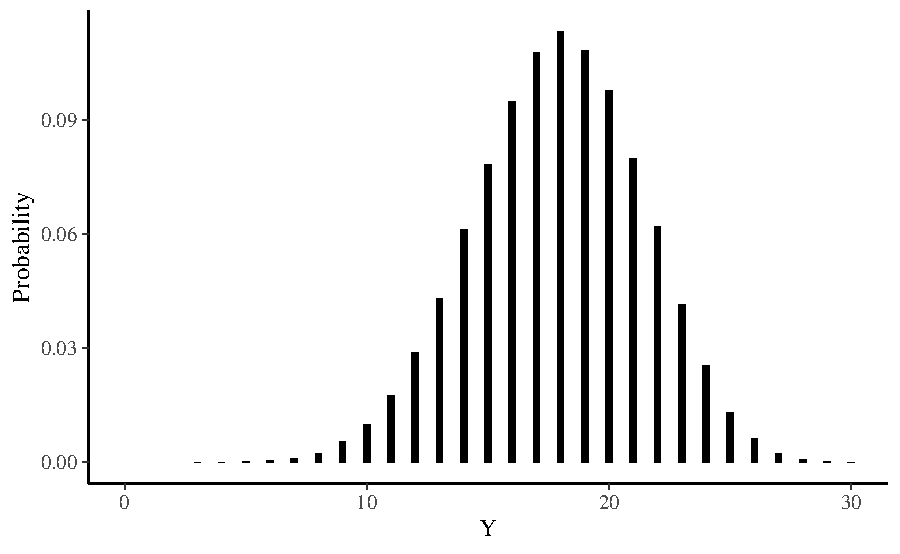
\includegraphics{ds4psy_files/figure-latex/unnamed-chunk-17-1} \end{center}

Infine, eseguendo la funzione \texttt{launch\_shinystan(fit)}, è possibile analizzare oggetti di classe \texttt{stanfit} mediante le funzionalità del pacchetto \texttt{ShinyStan}.

\hypertarget{interpretazione-dei-parametri}{%
\section{Interpretazione dei parametri}\label{interpretazione-dei-parametri}}

Assegnamo ai parametri la seguente interpretazione.

\begin{itemize}
\item
  L'intercetta pari a 25.9 indica il QI medio dei bamini la cui madre ha un QI = 0. Ovviamente questo non ha alcun significato. Vedremo nel modello successivo come trasformare il modello in modo da potere assegnare all'intercetta un'interpretazione sensata.
\item
  La pendenza di 0.61 indica che, all'aumentare di un punto del QI delle madri, il QI medio dei loro bambini aumenta di 0.61 unità. Se consideriamo la gamma di variazione del QI delle madri nel campione, il QI medio dei bambini cambia di 41 punti. Questo indica un sostanziale effetto del QI delle madri sul QI dei loro bambini: \((138.89 - 71.04) * 0.61 = 41.39\).
\item
  Il parametro \(\sigma\) = 18.3 fornisce una stima della dispersione delle osservazioni attorno al valore predetto dal modello lineare, ovvero fornisce una stima della deviazione standard dei residui attorno al valore atteso del modello lineare.
\end{itemize}

\hypertarget{centrare-i-predittori}{%
\subsection{Centrare i predittori}\label{centrare-i-predittori}}

Per migliorare l'interpretazione dell'intercetta possiamo ``centrare'' la \(x\), ovvero esprimere la \(x\) nei termini degli scarti dalla media: \(x - \bar{x}\). In tali circostanze, la pendenza della retta specificata dal modello lineare resta immutata, ma l'intercetta corrisponde a \(\E(y \mid x = \bar{x})\). Per ottenere questo risultato, modifichiamo i dati da passare a Stan:

\begin{Shaded}
\begin{Highlighting}[]
\NormalTok{data2\_list }\OtherTok{\textless{}{-}} \FunctionTok{list}\NormalTok{(}
  \AttributeTok{N =} \FunctionTok{length}\NormalTok{(df}\SpecialCharTok{$}\NormalTok{kid\_score),}
  \AttributeTok{y =}\NormalTok{ df}\SpecialCharTok{$}\NormalTok{kid\_score,}
  \AttributeTok{x =}\NormalTok{ df}\SpecialCharTok{$}\NormalTok{mom\_iq }\SpecialCharTok{{-}} \FunctionTok{mean}\NormalTok{(df}\SpecialCharTok{$}\NormalTok{mom\_iq)}
\NormalTok{)}
\end{Highlighting}
\end{Shaded}

Adattiamo il modello:

\begin{Shaded}
\begin{Highlighting}[]
\NormalTok{fit2 }\OtherTok{\textless{}{-}}\NormalTok{ mod}\SpecialCharTok{$}\FunctionTok{sample}\NormalTok{(}
  \AttributeTok{data =}\NormalTok{ data2\_list,}
  \AttributeTok{iter\_sampling =}\NormalTok{ 4000L,}
  \AttributeTok{iter\_warmup =}\NormalTok{ 2000L,}
  \AttributeTok{seed =}\NormalTok{ SEED,}
  \AttributeTok{chains =}\NormalTok{ 4L,}
  \AttributeTok{parallel\_chains =}\NormalTok{ 2L,}
  \AttributeTok{refresh =} \DecValTok{0}\NormalTok{,}
  \AttributeTok{thin =} \DecValTok{1}
\NormalTok{)}
\end{Highlighting}
\end{Shaded}

Trasformiamo l'oggetto \texttt{fit} in un oggetto di classe \texttt{stanfit}:

\begin{Shaded}
\begin{Highlighting}[]
\NormalTok{stanfit }\OtherTok{\textless{}{-}}\NormalTok{ rstan}\SpecialCharTok{::}\FunctionTok{read\_stan\_csv}\NormalTok{(fit2}\SpecialCharTok{$}\FunctionTok{output\_files}\NormalTok{())}
\end{Highlighting}
\end{Shaded}

Le stime a posteriori dei parametri si ottengono con

\begin{Shaded}
\begin{Highlighting}[]
\NormalTok{fit2}\SpecialCharTok{$}\FunctionTok{summary}\NormalTok{(}\FunctionTok{c}\NormalTok{(}\StringTok{"alpha"}\NormalTok{, }\StringTok{"beta"}\NormalTok{, }\StringTok{"sigma"}\NormalTok{))}
\CommentTok{\#\textgreater{} \# A tibble: 3 x 10}
\CommentTok{\#\textgreater{}   variable   mean median     sd    mad     q5    q95}
\CommentTok{\#\textgreater{}   \textless{}chr\textgreater{}     \textless{}dbl\textgreater{}  \textless{}dbl\textgreater{}  \textless{}dbl\textgreater{}  \textless{}dbl\textgreater{}  \textless{}dbl\textgreater{}  \textless{}dbl\textgreater{}}
\CommentTok{\#\textgreater{} 1 alpha    86.8   86.8   0.876  0.871  85.4   88.2  }
\CommentTok{\#\textgreater{} 2 beta      0.609  0.609 0.0591 0.0589  0.513  0.707}
\CommentTok{\#\textgreater{} 3 sigma    18.3   18.3   0.630  0.624  17.3   19.4  }
\CommentTok{\#\textgreater{} \# ... with 3 more variables: rhat \textless{}dbl\textgreater{},}
\CommentTok{\#\textgreater{} \#   ess\_bulk \textless{}dbl\textgreater{}, ess\_tail \textless{}dbl\textgreater{}}
\end{Highlighting}
\end{Shaded}

Si noti la nuova intercetta, ovvero 86.8. Questo valore indica il QI medio dei bambini le cui madri hanno un QI pari alla media del campione. Centrare i dati consente dunque di assegnare all'intercetta un'interpretazione utile.

\hypertarget{commenti-e-considerazioni-finali-1}{%
\section*{Commenti e considerazioni finali}\label{commenti-e-considerazioni-finali-1}}


La presente discussione suggerisce che è conveniente standardizzare i dati prima di procedere con l'analisi. Ciò può essere fatto all'interno del codice Stan (come negli esempi di questo Capitolo), oppure prima di passare i dati a Stan. Se vengono usati dati standardizzati diventa poi facile utilizzare distribuzioni a priori debolmente informative per i parametri. Tali distribuzioni a priori hanno, come unico scopo, quello di regolarizzare i dati e di facilitare la stima dei parametri mediante MCMC.

  \bibliography{refs.bib,book.bib,packages.bib}

\printindex

\end{document}
